\documentclass[../../main.tex]{subfiles}

\graphicspath{{../../image/}{../../figure/}}

\begin{document}

\section{基于图的机器学习}\label{section:ch13-基于图的机器学习}

我们可以使用图结构化数据来完成许多类型的应用，这些应用可以根据目标是预测节点、边还是整个图的属性来大致分组。节点预测（node prediction）的一个例子是根据文档之间的超链接和引用关系对文档进行主题分类。

对于边来说，举个例子，我们可能已知蛋白质网络中的一些相互作用，想要预测其他潜在的相互作用。这类任务称为边预测（edge prediction）或图补全（graph completion）任务。还有一些任务，其中边是已知的，我们的目标是在图中发现簇或“社群”。

最后一类是预测与整个图相关的属性。例如，我们可能希望预测特定分子是否能溶解于水。这里，我们得到的不是单个图，而是不同图的数据集，我们可以把它们看成从某个共同分布抽取而来，换句话说，我们假设图本身是独立同分布的（independent and identically distributed）。这类任务可以视为图回归（graph regression）或图分类（graph classification）任务。

对于分子溶解性分类的例子，我们可能会得到一个带标签的分子训练集，以及需要预测溶解性的新分子测试集。这是我们在前面章节中多次见到的典型归纳（inductive）任务的一个标准示例。然而，另一些图预测任务是直推式（transductive）的，我们得到整个图的结构以及一些节点的标签，要去预测剩余节点的标签。假设我们要区分一个大型社交网络中的每个用户节点是真实人物还是自动化机器人。在一个庞大且不断变化的社交网络中逐一核实并标注每个节点是不可行的，我们只能手工标注少数节点。因此，在训练期间，我们可以访问包含一部分节点标签的整个图，并试图预测剩余节点的标签。这是半监督学习的一种形式。

除了直接完成预测任务外，我们还可以在图上使用深度学习来发现有用的内部表示，这些表示随后可以促进一系列下游任务的完成。这称为图表示学习（graph representation learning）。例如，我们可以通过在大量分子结构语料库上训练深度学习系统来寻求构建分子的基础模型（foundation model）。这样的模型一旦训练成功，我们就可以通过使用小型标注数据集对它进行微调以完成各种特定任务。

图神经网络为每个节点定义了一个嵌入向量（embedding vector），该嵌入向量通常使用观测到的节点属性进行初始化，然后通过一系列可学习层进行转换，以创建学习表示。这与词嵌入或 token 在 Transformer 中的处理方式类似，通过一系列层的处理（参见\cref{chapter:ch12-Transformer与注意力机制}），便可以更好地捕获单词在文本其余部分上下文中的语义。图神经网络还可以学习表示图中每条边的特征向量（边嵌入）以及整个图的全局特征向量（图嵌入）。

\subsection{图的属性}\label{subsection:ch13-图的属性}

在本章中，我们将关注简单图，其中任意两个节点之间最多有一条边，边是无向的，并且没有连接到自身节点的环。这足以让我们介绍图神经网络的关键概念，同时也涵盖了图神经网络广泛的实际应用。这些概念之后可以应用于更复杂的图结构。

我们首先引入与图相关的一些符号，并定义一些重要的属性。

\begin{definition}[图、邻居与度]\label{definition:ch13-图}
一个图 $\mathcal{G}=(\mathcal{V},\mathcal{E})$ 由一组节点或顶点构成，用 $\mathcal{V}$ 表示，其中还包含一组边或连接，用 $\mathcal{E}$ 表示。我们用 $n=1,\cdots,N$ 来索引节点，并将从节点 $n$ 到节点 $m$ 的边写为 $(n,m)$。如果两个节点被一条边连接，则称它们为邻居节点，所有节点 $n$ 的邻居节点的集合用 $\mathcal{N}(n)$ 表示。节点 $n$ 的邻居节点的个数称为节点 $n$ 的度（degree），记作 $d_n\triangleq|\mathcal{N}(n)|$。
\end{definition}

% SUPPLEMENT: parent=definition:ch13-图; kind=motivation; location=紧随其后的 remark（重构新增）
\begin{remark}（重构新增）
把图写成二元组 $(\mathcal{V},\mathcal{E})$ 的意义在于把两类信息分开：$\mathcal{V}$ 只说“有哪些对象”，$\mathcal{E}$ 只说“谁与谁相连”，而后者正是图神经网络唯一能够利用的结构信息。这也解释了为什么后面的每一层都必须以邻接矩阵（或等价地，邻居集合 $\mathcal{N}(n)$）为输入之一：若只给出节点变量 $\bm{X}$，图就退化成一个无结构的集合，此时任何层都无法区分两个在 $\bm{X}$ 上相同、但在图中位置不同的节点。\par
本章的“简单图”假设包含三条子条件，它们各有各的作用。无向性给出 $A_{nm}=A_{mn}$，这是\cref{exercise:ch13-02}中“$\bm{A}^2$ 的对角元等于度”以及后面所有对称归一化写法的前提；无重边性使 $A_{nm}\in\{0,1\}$ 而不必取整数权，从而 $\sum_{m\in\mathcal{N}(n)}$ 与 $\sum_{m}A_{nm}$ 完全一致；无自环性给出 $A_{nn}=0$，于是 $\mathcal{N}(n)$ 不含 $n$ 本身——这一点在\eqref{align:ch13-简单更新}中会表现为“是否把节点自身并入求和”的显式区别。三条条件都不是数学上的必然要求，而是为了让记号在最简单的情形下保持干净；去掉其中任何一条，定义本身仍然成立，只是相应的公式需要改写。\par
度 $d_n$ 是本章反复使用的量：它在\eqref{align:ch13-更新算子}之后的初始化讨论中作为“节点没有观测数据”时的替代特征（度数独热向量），在\eqref{align:ch13-图卷积聚合}中作为对称归一化的分母，并在过度平滑的分析中刻画一个节点在一次消息传递中平均了多少条边。度只依赖 $\mathcal{E}$，与 $\bm{X}$ 无关，因此它是纯粹的结构量。
\end{remark}

除了图结构，通常还有与节点相关联的观测数据。

\begin{definition}[节点变量与数据矩阵]\label{definition:ch13-节点数据矩阵}
对于每个节点 $n$，我们可以将相应的节点变量表示为一个 $D$ 维的列向量 $\bm{x}_n$，将这些变量组合成一个 $N\times D$ 维的数据矩阵 $\bm{X}$，其中第 $n$ 行由 $\bm{x}_n^{\mathsf T}$ 表示。
\end{definition}

% SUPPLEMENT: parent=definition:ch13-节点数据矩阵; kind=motivation; location=紧随其后的 remark（重构新增）
\begin{remark}（重构新增）
这里把 $N$ 个节点变量堆叠成 $\bm{X}\in\mathbb{R}^{N\times D}$ 而不是保留为列表，是为了让“按节点作用”的变换可以写成矩阵乘法。行索引与 $\bm{A}$ 的行索引使用同一套编号，这一点是后面的矩阵形式\eqref{align:ch13-习题矩阵形式}能够成立的前提：只有当 $\bm{X}$ 的第 $n$ 行、$\bm{A}$ 的第 $n$ 行、第 $n$ 列都指向同一个节点时，$\bm{A}\bm{H}$ 的第 $n$ 行才会恰好是节点 $n$ 的邻居聚合量。\par
特征维数 $D$ 与节点数 $N$ 是两个独立的量：$D$ 由数据决定，$N$ 由具体的图决定。正因为网络的参数只作用在 $D$ 维向量上而不依赖 $N$，同一个图神经网络才能处理节点数不同的图，这正是\cref{section:ch13-神经信息传递}开头所说的“变长输入”能力。\par
需要强调的是，$\bm{X}$ 的行顺序完全由我们给节点指定的编号决定，而这个编号是任意的。\eqref{align:ch13-置换不变性}与\eqref{align:ch13-置换等变性}要刻画的就是“网络的输出不应依赖这个任意选择”。
\end{remark}

图中的边也可能与数据变量相关联，但在当下我们只关注节点变量（参见\cref{subsection:ch13-边嵌入}）。

\subsection{邻接矩阵}\label{subsection:ch13-邻接矩阵}

指定图中边的一种便捷方式是使用邻接矩阵。

\begin{definition}[邻接矩阵]\label{definition:ch13-邻接矩阵}
邻接矩阵（adjacency matrix）用 $\bm{A}$ 表示。要定义邻接矩阵，我们首先需要为节点分配一个顺序。如果图中有 $N$ 个节点，我们可以使用 $n=1,\cdots,N$ 来索引它们。邻接矩阵的维度是 $N\times N$，在其中的每个元素位置 $n,m$，只要从节点 $n$ 到节点 $m$ 的边存在，就在该处填入 $1$，所有其他元素位置都填入 $0$。对于具有无向边的图，邻接矩阵是对称的，因为存在从节点 $n$ 到节点 $m$ 的边意味着也存在从节点 $m$ 到节点 $n$ 的边，对于所有的 $n$ 和 $m$，都有 $A_{nm}=A_{mn}$。
\end{definition}

% SUPPLEMENT: parent=definition:ch13-邻接矩阵; kind=motivation; location=紧随其后的 remark（重构新增）
\begin{remark}（重构新增）
邻接矩阵把 $\mathcal{E}$ 编码成一个 $N\times N$ 的数值数组，代价是引入了对节点编号的依赖：同一个图换一种编号方式，得到的矩阵并不相同，而是相差一个相似变换（见\eqref{align:ch13-邻接矩阵置换}）。这个代价是必须付的，因为神经网络只能接收数值数组；而它带来的问题正是下一小节“置换等变性”要解决的。\par
定义中的三条约定都可以在矩阵上读出：$A_{nm}=A_{mn}$ 对应无向，$A_{nn}=0$ 对应无自环，$A_{nm}\in\{0,1\}$ 对应无重边。若是一般图，则 $A_{nm}$ 可以取边权，$A_{nn}$ 可以非零，$A_{nm}\neq A_{mn}$ 表示有向边——这些推广都不改变后面的公式，只改变 $\bm{A}$ 的性质。\par
按定义直接计算，$\bm{A}^2$ 的 $(n,m)$ 元等于从 $n$ 到 $m$ 的长度为 $2$ 的路径条数；特别地，对角元 $(\bm{A}^2)_{nn}$ 恰是节点 $n$ 的度（见\cref{exercise:ch13-02}）。这说明度并非额外引入的量，它已经隐含在 $\bm{A}$ 中。
\end{remark}

邻接矩阵的一个例子如\cref{figure:ch13-邻接矩阵例子}所示。

\begin{figure}[htbp]
  \centering
  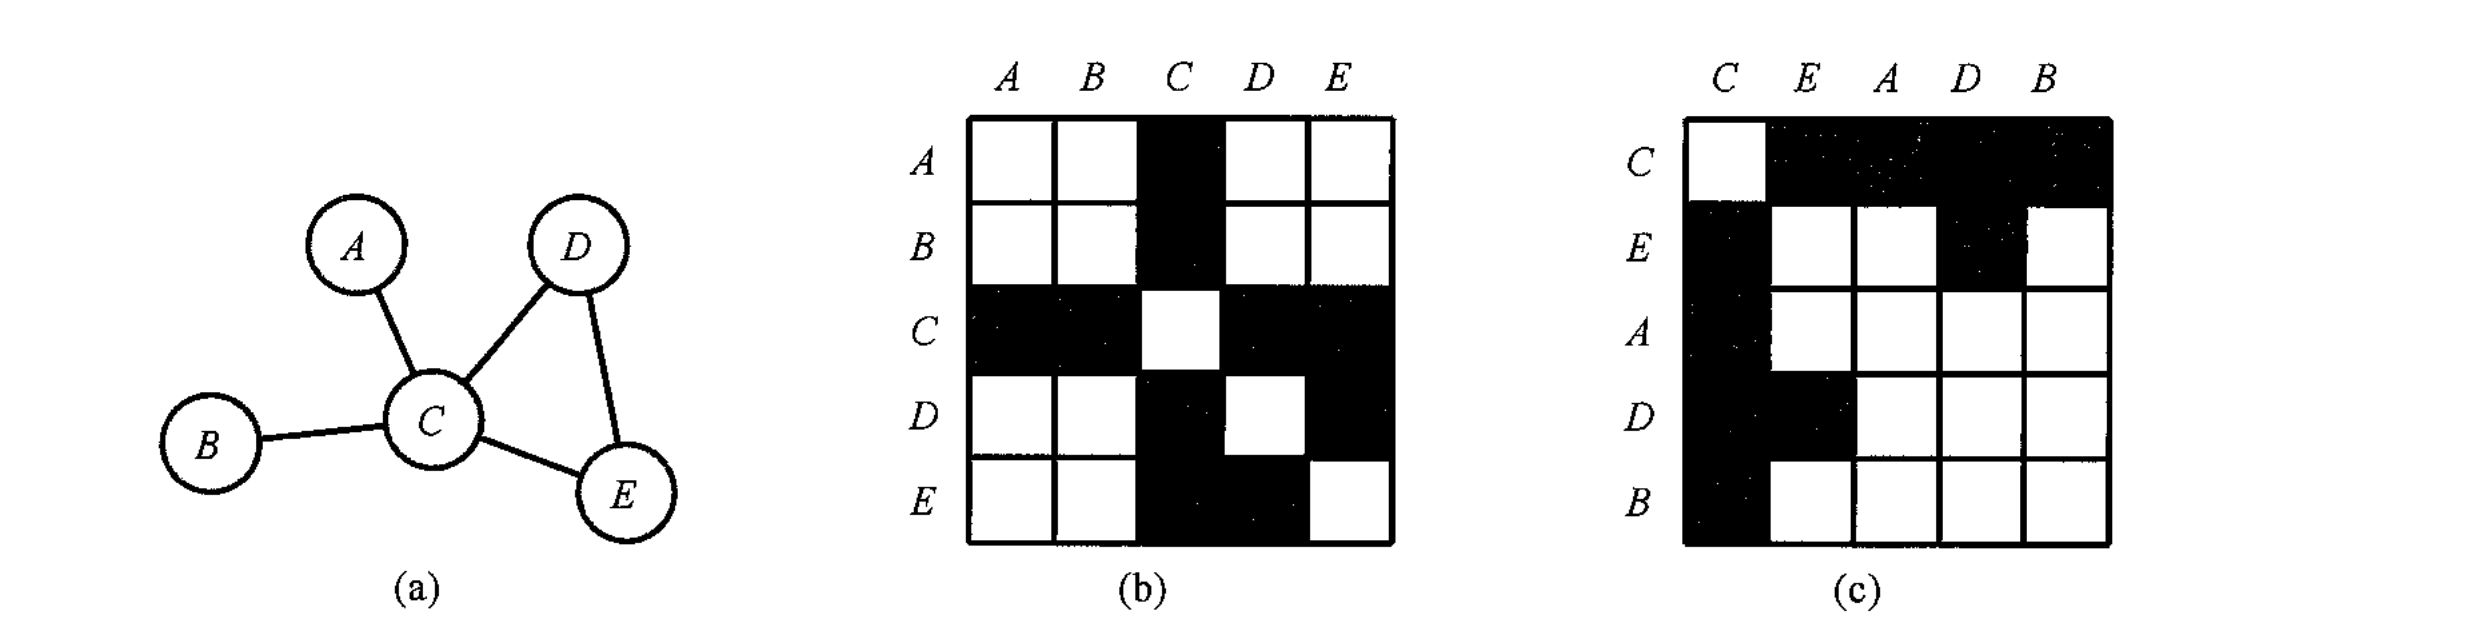
\includegraphics[width=0.95\textwidth]{ch13-fig13.2-adjacency.png}
  \caption{邻接矩阵的一个例子：(a) 一个包含 5 个节点的图；(b) 对应于特定节点顺序的邻接矩阵；(c) 对应于另一不同节点顺序的邻接矩阵}
  \label{figure:ch13-邻接矩阵例子}
\end{figure}

邻接矩阵定义了图的结构，我们可以考虑直接将其作为神经网络的输入。为此，我们可以“展平”邻接矩阵，例如将列连接成一个长的列向量。然而，这种方法的一个主要问题在于邻接矩阵取决于节点排序的任意选择，如\cref{figure:ch13-邻接矩阵例子}所示。假设我们想要预测一个分子的溶解性，这显然不应该取决于写下邻接矩阵时给节点分配的顺序。由于节点的排序方式的数量随节点数的增加而阶乘式增长，尝试通过使用大数据集或数据增强来学习置换不变性是不切实际的。相反，在构建网络架构时，我们应当将这种不变性视为归纳偏置。

\subsection{置换等变性}\label{subsection:ch13-置换等变性}

我们可以引入置换矩阵 $\bm{P}$ 的概念，以便在数学上表达节点标签的排列。

\begin{definition}[置换矩阵]\label{definition:ch13-置换矩阵}
置换矩阵与邻接矩阵大小相同，并指定了节点排序的特定排列。置换矩阵在每行和每列中各含有一个 $1$，其余元素都是 $0$，于是置换矩阵中元素位置 $n,m$ 的 $1$ 表示节点 $n$ 在重新排列后将标记为 $m$。例如，考虑从 $(A,B,C,D,E)$ 到 $(C,E,A,D,B)$ 的排列，它对应于\cref{figure:ch13-邻接矩阵例子}中的两种节点排序选择。相应的置换矩阵形式为（见\cref{exercise:ch13-01}）
\begin{align}
\bm{P}=\begin{pmatrix}0&0&1&0&0\\0&0&0&0&1\\1&0&0&0&0\\0&0&0&1&0\\0&1&0&0&0\end{pmatrix}.
\label{align:ch13-置换矩阵例子}
\end{align}
我们可以更加正式地定义置换矩阵如下。首先引入标准单位向量 $\bm{u}_n$，其中 $n=1,\cdots,N$。这是一个列向量，其中除了第 $n$ 个元素等于 $1$ 之外，其他所有元素都等于 $0$。在这种表示法中，单位矩阵如下所示：
\begin{align}
\bm{I}=\begin{pmatrix}\bm{u}_1^{\mathsf T}\\\bm{u}_2^{\mathsf T}\\\vdots\\\bm{u}_N^{\mathsf T}\end{pmatrix}.
\label{align:ch13-单位矩阵}
\end{align}
引入一个置换函数 $\pi(\cdot)$，将 $n$ 映射到 $m=\pi(n)$。对应的置换矩阵如下所示：
\begin{align}
\bm{P}=\begin{pmatrix}\bm{u}_{\pi(1)}^{\mathsf T}\\\bm{u}_{\pi(2)}^{\mathsf T}\\\vdots\\\bm{u}_{\pi(N)}^{\mathsf T}\end{pmatrix}.
\label{align:ch13-置换矩阵一般形式}
\end{align}
\end{definition}

% SUPPLEMENT: parent=definition:ch13-置换矩阵; kind=motivation; location=紧随其后的 remark（重构新增）
\begin{remark}（重构新增）
按\eqref{align:ch13-置换矩阵一般形式}定义的 $\bm{P}$ 的行是标准基向量，因此 $\bm{P}$ 是正交矩阵：$\bm{P}^{\mathsf T}\bm{P}=\bm{P}\bm{P}^{\mathsf T}=\bm{I}$。这一点在后面反复使用——\eqref{align:ch13-邻接矩阵置换}中的 $\bm{P}^{\mathsf T}$ 是 $\bm{P}$ 的逆，\eqref{align:ch13-层等变性}中的 $\bm{P}\bm{A}\bm{P}^{\mathsf T}$ 保持 $\bm{A}$ 的对称性与特征值，\cref{theorem:ch13-图网络等变性}的证明中对网络整体的归纳也依赖 $\bm{P}^{\mathsf T}\bm{P}=\bm{I}$。\par
置换函数 $\pi$ 的读法是“节点 $n$ 在重新编号之后被叫作 $\pi(n)$”。由于 $\bm{P}$ 的第 $i$ 行是 $\bm{u}_{\pi(i)}^{\mathsf T}$，矩阵 $\bm{P}\bm{X}$ 的第 $i$ 行就等于 $\bm{X}$ 的第 $\pi(i)$ 行（见\cref{exercise:ch13-04}）：新矩阵的第 $i$ 行记录的是“新编号为 $i$ 的那个节点”的旧数据。$\pi$ 必须是 $\{1,\cdots,N\}$ 到自身的双射，因此全体置换矩阵构成一个群（对称群 $S_N$ 的矩阵表示），“对任意 $\bm{P}$ 成立”这句话才有确切含义。\par
以\eqref{align:ch13-置换矩阵例子}为例，$\pi(1)=3,\pi(2)=5,\pi(3)=1,\pi(4)=4,\pi(5)=2$，即编号 $1,2,3,4,5$（对应 $A,B,C,D,E$）在新编号下依次成为 $3,5,1,4,2$，于是新序列按 $1$ 到 $5$ 读出的节点是 $C,E,A,D,B$，与题设一致。把 $\bm{P}$ 作用在\cref{figure:ch13-邻接矩阵例子}(b) 的邻接矩阵上，就得到同一图的 (c)。
\end{remark}

当我们重新排序一个图的节点上的标签时，对应的节点数据矩阵 $\bm{X}$ 的效果是根据 $\pi(\cdot)$ 进行置换操作，这可以通过在其前面乘上 $\bm{P}$ 来实现（见\cref{exercise:ch13-04}），即
\begin{align}
\widetilde{\bm{X}}=\bm{P}\bm{X}.
\label{align:ch13-数据矩阵置换}
\end{align}
对于邻接矩阵，行和列都会被置换。同样，行可以通过在前面乘上 $\bm{P}$ 来置换，而列可以通过在后面乘上 $\bm{P}^{\mathsf T}$ 来置换（见\cref{exercise:ch13-05}），从而得到一个新的邻接矩阵：
\begin{align}
\widetilde{\bm{A}}=\bm{P}\bm{A}\bm{P}^{\mathsf T}.
\label{align:ch13-邻接矩阵置换}
\end{align}

当我们将深度学习应用于图结构化数据时，需要以数值形式表示图结构，这样才能将它们输入神经网络，这就要求我们为节点指定顺序。然而，我们选择的具体节点排序是任意的，所以必须确保图的任何全局属性不依赖于这种排序方式。

\begin{definition}[置换不变性与置换等变性]\label{definition:ch13-不变性与等变性}
设 $y(\cdot,\cdot)$ 是网络的输出。网络预测必须对节点标签的重新排序具有不变性，即
\begin{align}
y(\widetilde{\bm{X}},\widetilde{\bm{A}})=y(\bm{X},\bm{A})\qquad\text{不变性}
\label{align:ch13-置换不变性}
\end{align}
其中 $y(\cdot,\cdot)$ 是网络的输出。有些情况下，我们要对单个节点进行预测。在这种情况下，如果我们重新排序节点标签，则相应的预测应显示相同的次序，这样不论如何选择顺序，给定的预测总是与同一个节点相关联。换言之，节点级预测应该对节点标签重新排序保持等变性，即
\begin{align}
\bm{y}(\widetilde{\bm{X}},\widetilde{\bm{A}})=\bm{P}\,\bm{y}(\bm{X},\bm{A})\qquad\text{等变性}
\label{align:ch13-置换等变性}
\end{align}
其中 $\bm{y}(\cdot,\cdot)$ 是网络输出的一个向量，每个节点对应其中的一个元素。
\end{definition}

% SUPPLEMENT: parent=definition:ch13-不变性与等变性; kind=motivation; location=紧随其后的 remark（重构新增）
\begin{remark}（重构新增）
不变性与等变性是两个强度不同的要求，适用对象也不同。当网络的输出是一个与整张图关联的量（例如分子是否溶于水）时，输出中没有“节点”这一维度，重排节点不应改变任何东西，这就是\eqref{align:ch13-置换不变性}；当输出是逐节点的（例如每个用户是否为机器人）时，输出本身是一个 $N$ 维向量，重排节点会使输出向量的分量跟着换位，但“第 $n$ 个节点的预测”必须还是同一个数，这就是\eqref{align:ch13-置换等变性}。若把二者混淆——例如要求节点级输出不变——就会得到荒谬的结论：重排之后第 $1$ 个分量的含义已经变成了另一个节点。\par
两式中的 $\bm{P}$ 必须是同一个任意置换矩阵，且必须同时作用在 $\bm{X}$ 与 $\bm{A}$ 上。只置换 $\bm{X}$ 而不置换 $\bm{A}$（或反之）描述的是“换了一种节点特征顺序但仍沿用旧图”，那不是同一个图的重排，因而不能作为对称性要求。\par
两个要求之间有确定的联系：若 $\bm{y}$ 是等变的，则任何对分量求和（或取平均、取最大）的读出函数都给出不变的输出，因为 $\sum_n(\bm{P}\bm{y})_n=\sum_n y_n$。这正是\cref{subsection:ch13-图分类}中用求和构造图级预测的依据，也说明“等变”是比“不变”更基本的要求。\par
最后要注意，\eqref{align:ch13-置换不变性}与\eqref{align:ch13-置换等变性}是网络应当满足的性质，而不是可以自动成立的事实：把 $\bm{A}$ 展平后送入多层感知机所得到的函数一般不满足它们，因此必须把对称性写进架构，这正是\cref{section:ch13-神经信息传递}的出发点。
\end{remark}

\end{document}
